

\chapter{Identification Schemes}

\section{How to prove yourself}
    \begin{itemize}
        \item Basic Problem: Access Control
        \item How do you prove that you have the credentials to access?
        \item Passwords?
        \item Replay Attacks!
    \end{itemize}
    \begin{center}
	    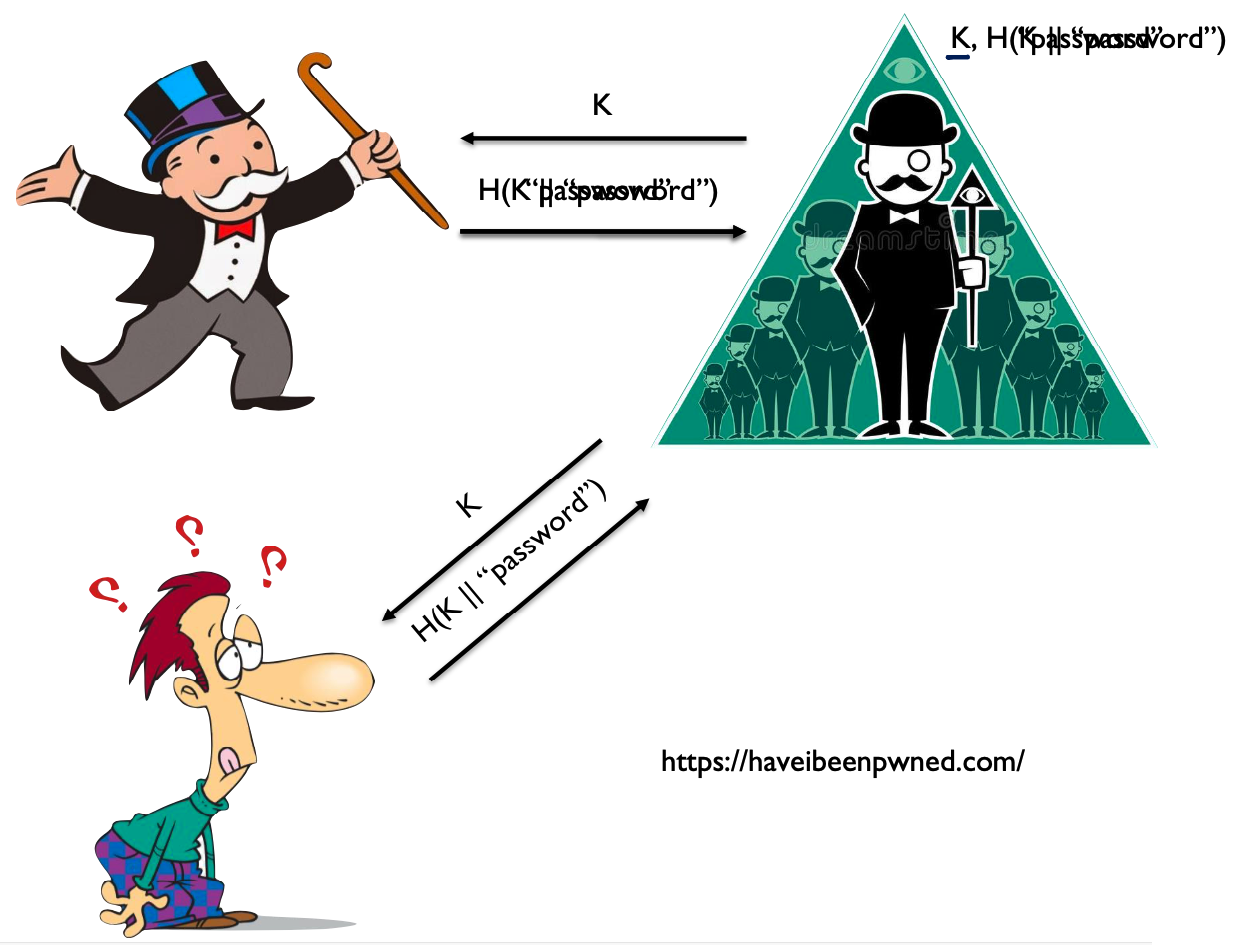
\includegraphics[width=160mm]{Graphics/Digital Signatures/is1.png}
    \end{center}

\section{Identification Schemes}
    \begin{center}
	    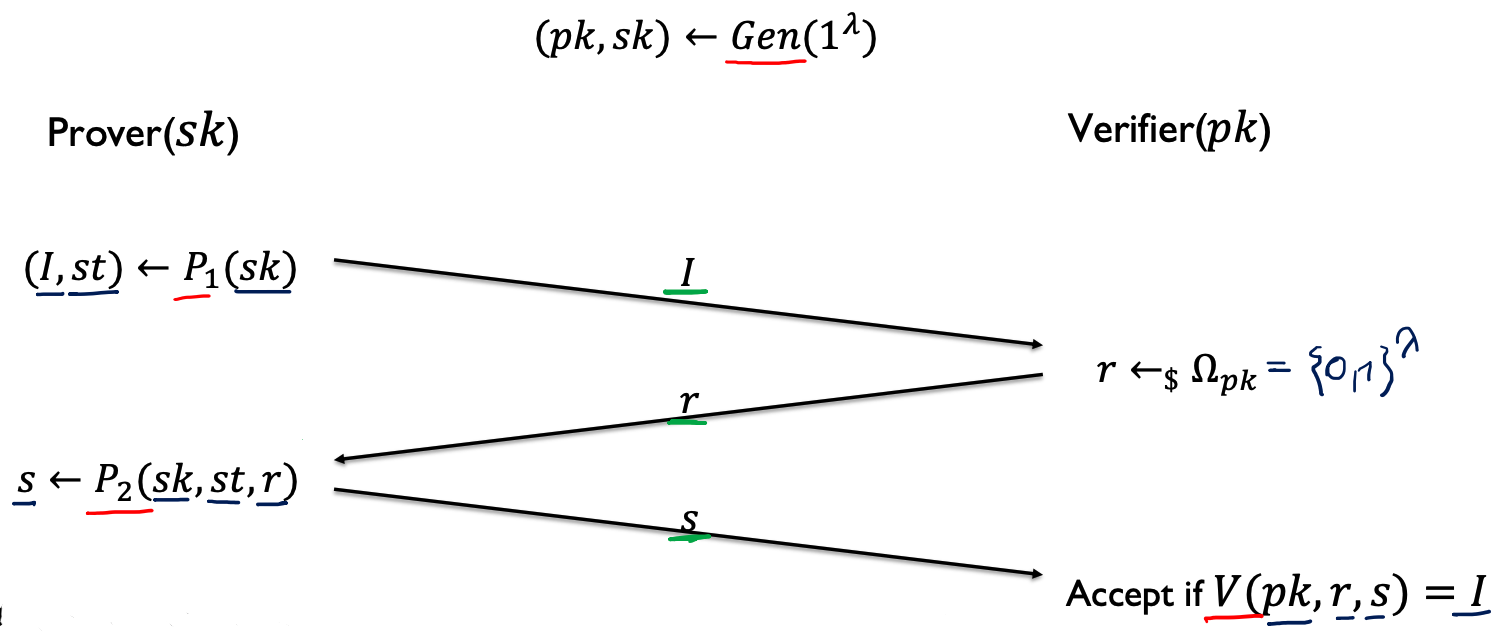
\includegraphics[width=160mm]{Graphics/Digital Signatures/is2.png}
    \end{center}
    \begin{itemize}
        \item Completeness: Verifier accepts with probability 1 for honest runs
        \item A public transcript consists of $(I,r,s)$.
        \item Let $trans(pk,sk)$ be (randomized) algorithm which generates transcripts of protocol runs
    \end{itemize}

\section{Security of Identification Schemes}
    \begin{definition}
        An identification scheme $(Gen,P_1,P_2,V)$ is \textbf{secure}, if it holds for \textbf{every PPT-adversary} $\mathcal{A}$ 
        there exists a negligible function $v$ s.t. for all $\lambda \in \mathbb{N}$
        $$Pr[Ident_{\mathcal{A}}(\lambda)=1] < v(\lambda)$$
    \end{definition}
    \begin{center}
	    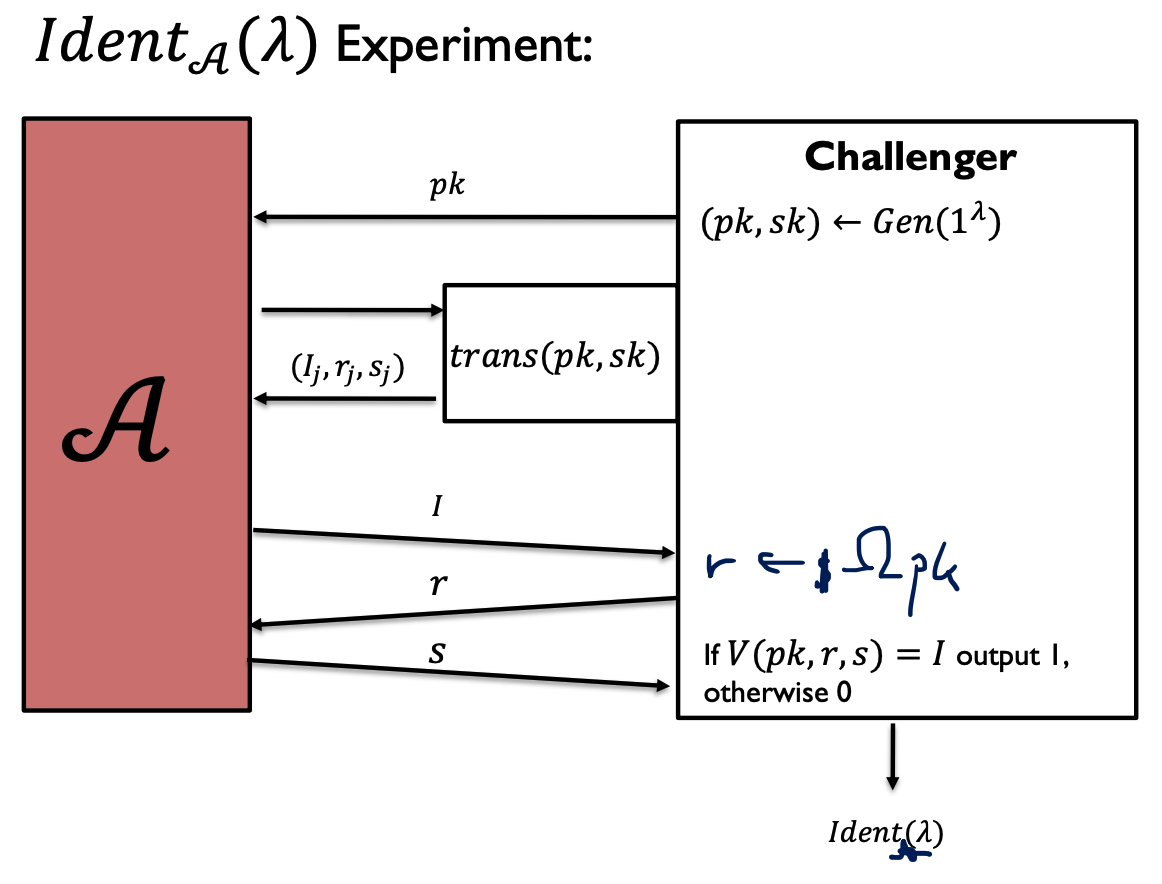
\includegraphics[width=140mm]{Graphics/Digital Signatures/is3.png}
    \end{center}

\section{Recap: The Discrete Logarithm Problem}
    \begin{itemize}
        \item Let $\mathbb{G}$ be a cryptographic group of order $p$ with generator $g$
        \item We omit group generation algorithm, but bear in mind that this is actually an infinite family of groups
        \item The discrete logarithm assumption in $\mathbb{G}$ conjectures that it holds for every PPT algorithm $\mathcal{A}$ that
        $$Pr[\mathcal{A}(g^x)=x] \leq negl(\lambda)$$
        where the probability is taken over the random choice of $x \leftarrow_{\$} \mathbb{Z}_p$
    \end{itemize}

\section{Schnorr's Identification Scheme}
    \begin{center}
	    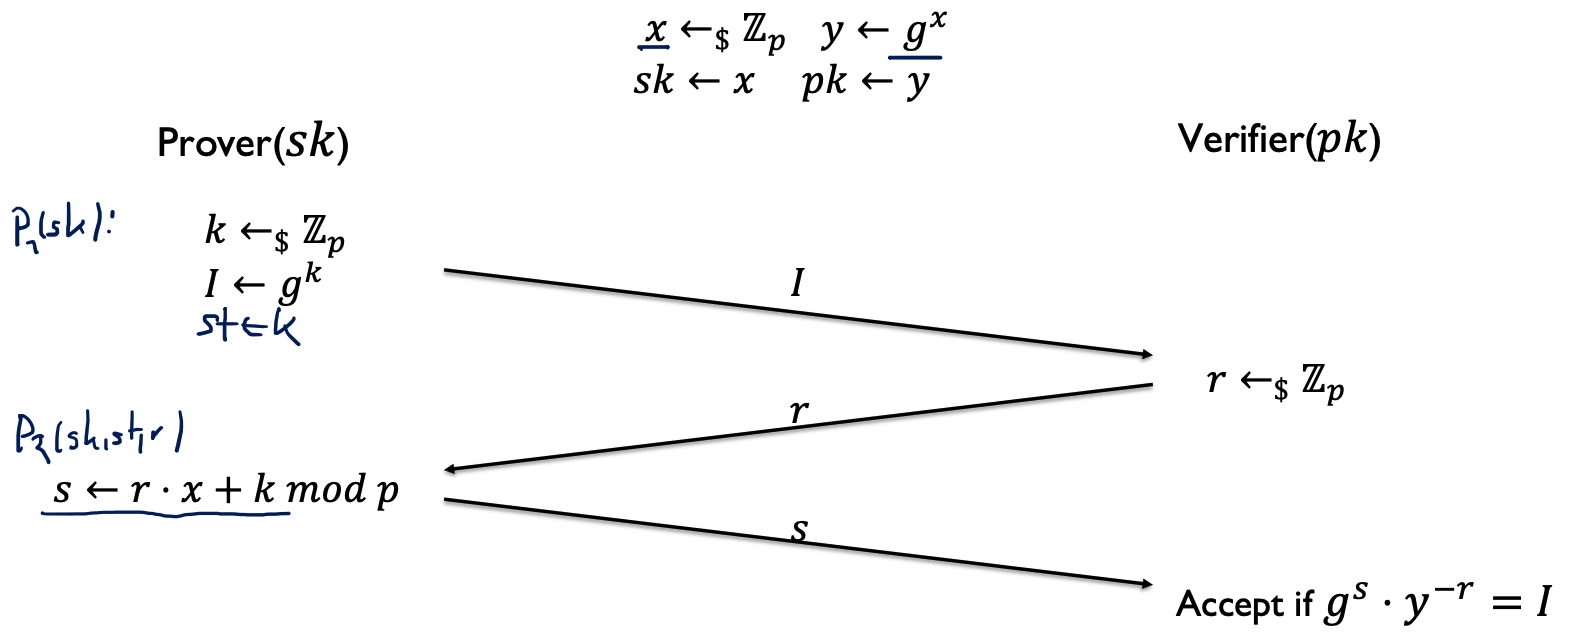
\includegraphics[width=140mm]{Graphics/Digital Signatures/is4.png}
    \end{center}
    $$g^{r \cdot x + k} \cdot y^{-r} = (g^x)^r \cdot g^k \cdot y^{-r} = y^r \cdot g^k \cdot y^{-r} = g^k = I$$

\newpage
\section{Security}
    \begin{theorem}\label{thm9.2}
        \begin{itemize}
            \item Assume that the discrete logarithm assumption holds in the grouop $\mathbb{G}$
            \item Then the Schnorr Identification Scheme is secure
        \end{itemize}
    \end{theorem}
    \begin{proof}
        Let $\mathcal{A}$ be a PPT adversary with non-negligible advantage $\epsilon$ against $(Gen,P_1,P_2,V)$
        $$Pr[Ident_{\mathcal{A}}=1] \geq \epsilon$$
        \begin{center}
	        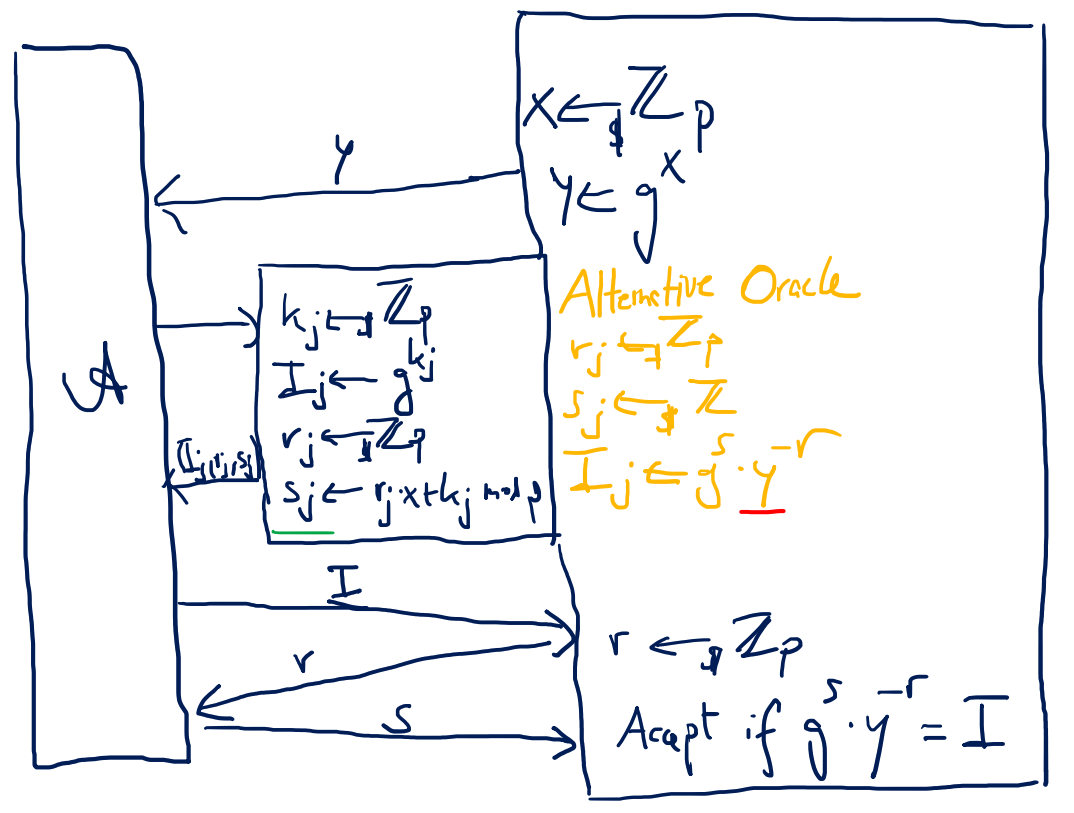
\includegraphics[width=120mm]{Graphics/Digital Signatures/is5.png}
        \end{center}
        Construct adversary $\mathcal{A}$' against DLOG
        \begin{center}
	        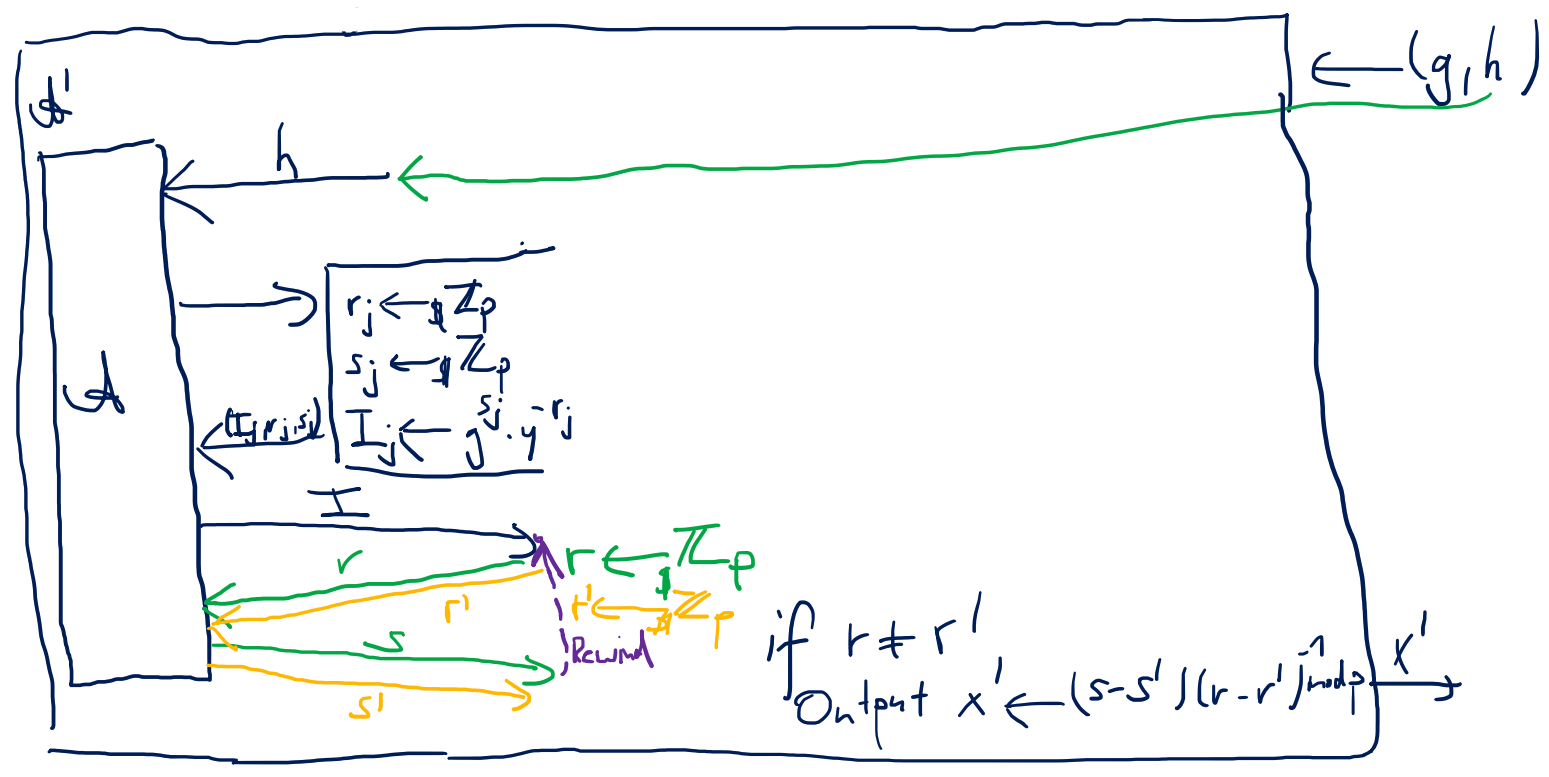
\includegraphics[width=140mm]{Graphics/Digital Signatures/is6.png}
        \end{center}
        Both $(I,r,s)$ and $(I,r',s')$ are accepted
        \begin{align*}
            [I=g^s \cdot h^{-r} \wedge I=g^{s'} \cdot h^{-r'}] &\Rightarrow g^s \cdot h^{-r} = g^{s'} \cdot h^{-r'}\\
            &\Rightarrow g^{s-s'} = h^{r-r'}\\
            &\Rightarrow h = g^{\frac{s-s'}{r-r'}} = g^{x'}
        \end{align*}
        From the view of $\mathcal{A}$, $\mathcal{A}$' simulates the Ident-experiment faithfully for both runs.\\\\
        \textbf{\underline{However:}} The two runs are \underline{not} independent!\\
        Let $z$ be a random variable which incorporates all random choices in the $Ident$-experiment 
        \underline{except} the choice of $r$.
        Write $Ident_{\mathcal{A}}(\lambda) = Exp(z,r)$.
        It holds that 
        \begin{align*}
            \epsilon \leq Pr[Ident_{\mathcal{A}}(\lambda)=1] &= Pr_{z,r}[Exp(z,r)=1]\\
            &= \sum\limits_{\xi}Pr[Exp(z,r)=1 \mid z=\xi] \cdot Pr[z=\xi]\ \ \ \text{(LOTP)}\\
            &= \sum\limits_{\xi}\underbrace{Pr[Exp(\xi,r)=1]}_{\epsilon_{\xi}} \cdot Pr[z=\xi]\\
            &= E_{\xi}[\epsilon_{\xi}]
        \end{align*}
        With $\epsilon_{\xi} = Pr[Exp(\xi,r)=1]$ defined as random variable.\\
        And with Jensen's inequality it holds: $E[\epsilon^2_{\xi}] \geq E[\epsilon_{\xi}]^2$
        \begin{align*}
            Pr[\mathcal{A}'(g,g^x)=x] &\geq Pr_{z,r,r'}[Exp(z,r)=1 \wedge Exp(z,r')=1 \wedge r \neq r']\\
            &\geq Pr_{z,r,r'}[Exp(z,r)=1 \wedge Exp(z,r')=1] - \underbrace{Pr[r = r']}_{= \frac{1}{p}}\\
            &= \sum\limits_{\xi} Pr[z=\xi] \cdot Pr_{r,r'}[Exp(\xi,r)=1 \wedge Exp(\xi,r')=1] - \frac{1}{p}\ \ \ \text{(LOTP)}\\
            &= \sum\limits_{\xi} Pr[z=\xi] \cdot \underbrace{Pr_{r}[Exp(\xi,r)=1]}_{\epsilon_{\xi}} \cdot \underbrace{Pr_{r'}[Exp(\xi,r')=1]}_{\epsilon_{\xi}} - \frac{1}{p}\\
            &= \sum\limits_{\xi} Pr[z=\xi] \cdot {\epsilon_{\xi}}^2 - \frac{1}{p}\\
            &= E_{\xi}[\epsilon^2_{\xi}] - \frac{1}{p}
            \geq E_{\xi}[\epsilon_{\xi}]^2 - \frac{1}{p} = \epsilon^2 - \underbrace{\frac{1}{p}}_{negl.}
        \end{align*}
        which is non-negligible.\\
        $\Rightarrow$ Contradicts the PLOG assumption!
    \end{proof}

\section{Summary}
    \begin{itemize}
        \item Naive attempts for access control are often susceptible to replay attacks
        \item Identification schemes provide security against replay attacks
        \item The Schnorr identification scheme is secure under the discrete logarithm assumption
    \end{itemize}


